\section{Today's assignment}
Today's class delves into multimodal architectures, focusing on how models learn the relationships between different types of data, including images and text. More specifically, we will explore \textbf{CLIP (Contrastive Language-Image Pre-Training)} \cite{clip_multimodal_day}: a foundational model that learns visual concepts from natural language supervision through a shared embedding space. CLIP's shared embedding space has heavily influenced modern large-scale multimodal systems, stemming from its initial application to models like \href{https://openai.com/index/dall-e/}{DALL-E}. As a means of encoding textual prompts and conditioning image synthesis, it enables text-driven image generation and manipulation, while also facilitating the ranking of generative outputs.

On that note, the primary focus of this class is to complete this lab's notebook (adapted from a \href{https://github.com/huggingface/transformers/blob/f4fc42216cd56ab6b68270bf80d811614d8d59e4/src/transformers/models/clip/modeling_clip.py#L860}{HuggingFace PyTorch implementation of CLIP}) sustaining the following milestones: (i) understand CLIP's dual-encoder architecture and contrastive learning, (ii) encode images and captions into the shared embedding space of CLIP, (iii) implement a zero-shot rescoring pipeline by sampling candidate sentences, computing CLIP similarity scores, and selecting the best match, and (iv) visualizing resulting image-text distances of a Gemma \textbf{Vision-Language Model (VLM)} and how cross-modal tokenization and convolution play a role.

By the end of this session, you'll have hands-on experience with the core mechanics that make CLIP and many other multimodal systems so powerful.

%\paragraph{TODO}
%\begin{itemize}
    %\item Update the chapter with the code and %implementation details developed by others in the team (se far I have kept some simple code example using %huggingfaces and typical things)
    %\item Review and consider expand on the mathematical %details
%    \item Review the ordering of topics and details
    %\item Create correct illustration to \verb|%includegraphics|
    %\item Include citation and better literature review of %models
%\end{itemize}
%For this, we will utilize the Hugging Face \texttt{transformers} library to combine a pre-trained language model with CLIP's powerful image and text encoders, thereby building a visually aware system.

\section{Before Diving into Multimodal Models}
Before building our model, it is essential first to understand the core concepts that make multimodal learning possible.

\subsection{Image Tokenization: From Pixels to Patches}
\label{subsec:vit_stuff}
Transformers operate on sequences of inputs. In the case of natural language, as we have seen in the previous day, this involves breaking text into smaller pieces through tokenization. A similar concept is required for images: we partition a grid of pixels into a sequence of patches and feed them into a Vision Transformer (ViT) \cite{vit_multimodal_day}. This process, visually demonstrated in Figure~\ref{fig:vit_diagram}, works through the following sequence of operations:
\begin{enumerate}
    \item \textbf{Patch Extraction and Flatenning:} With an input image \(x \in \mathbb{R}^{H \times W \times C}\) (where \(H\) and \(W\) are the height and width of the image in pixels, respectively, and \(C\) is the number of color channels per pixel), split it into a sequence of flattened non-overlapping patches (\(x_p \in \mathbb{R}^{N \times (P^2 \cdot C)}\)), where:
    \begin{align}
        N = \frac{H}{P} \times \frac{W}{P}
    \end{align}
     is the resulting number of patches, each of size \(P \times P\) (e.g., \(16 \times 16\) pixels), and where each flattened patch is a one-dimensional vector \(x_p\), where:
    \begin{align}
        x_p = 
        \bigl[p_{1,1,1},\, p_{1,1,2},\, p_{1,1,3},\, p_{1,2,1},\, p_{1,2,2},\, p_{1,2,3},\,\dots \bigr]^\top
        \;\in\;\mathbb{R}^{P^2 \cdot C}
    \end{align}
    These are then treated as "tokens", similarly to word tokens of standard transformers;
    \item \textbf{Linear Projection to Embeddings:} Apply a learnable linear layer (\(E \in \mathbb{R}^{(P^2 \cdot C) \times D}\)) to each flattened patch to project each patch into a \(D\)-dimensional embedding space, such that:
    \begin{align}\label{eq:linear_projection}
        x_p^{(i)} = x_p^{(i)}E\quad\in\mathbb{R}^D
    \end{align}

    \item \textbf{Class Token and Positional Embeddings:} Prepend a learnable class embedding (\(z_0^0 = x_{class} \in \mathbb{R}^D\)), whose final state (\(z_L^0\)) will represent the entire image, and, just like text-based transformers, add a learnable one-dimensional positional embedding (\(E_{pos} \in \mathbb{R}^{(N+1) \times D}\)) to retain spatial information about where each patch was located in the original image, such that:
    \begin{align}\label{eq:class_token_positional_embeddings}
          z^0 = [x_{class}; x_p^{(1)}E; x_p^{(2)}E;...; x_p^{(N)}E] + E_{pos}
    \end{align}

    \item \textbf{Transformer Encoder:} Feed the previous sequence into a standard transformer encoder of \(L\) layers, enabling the self-attention mechanism to weigh the importance of different parts of the image relative to one another.
\end{enumerate}
\begin{figure}[h!]
	\centering
    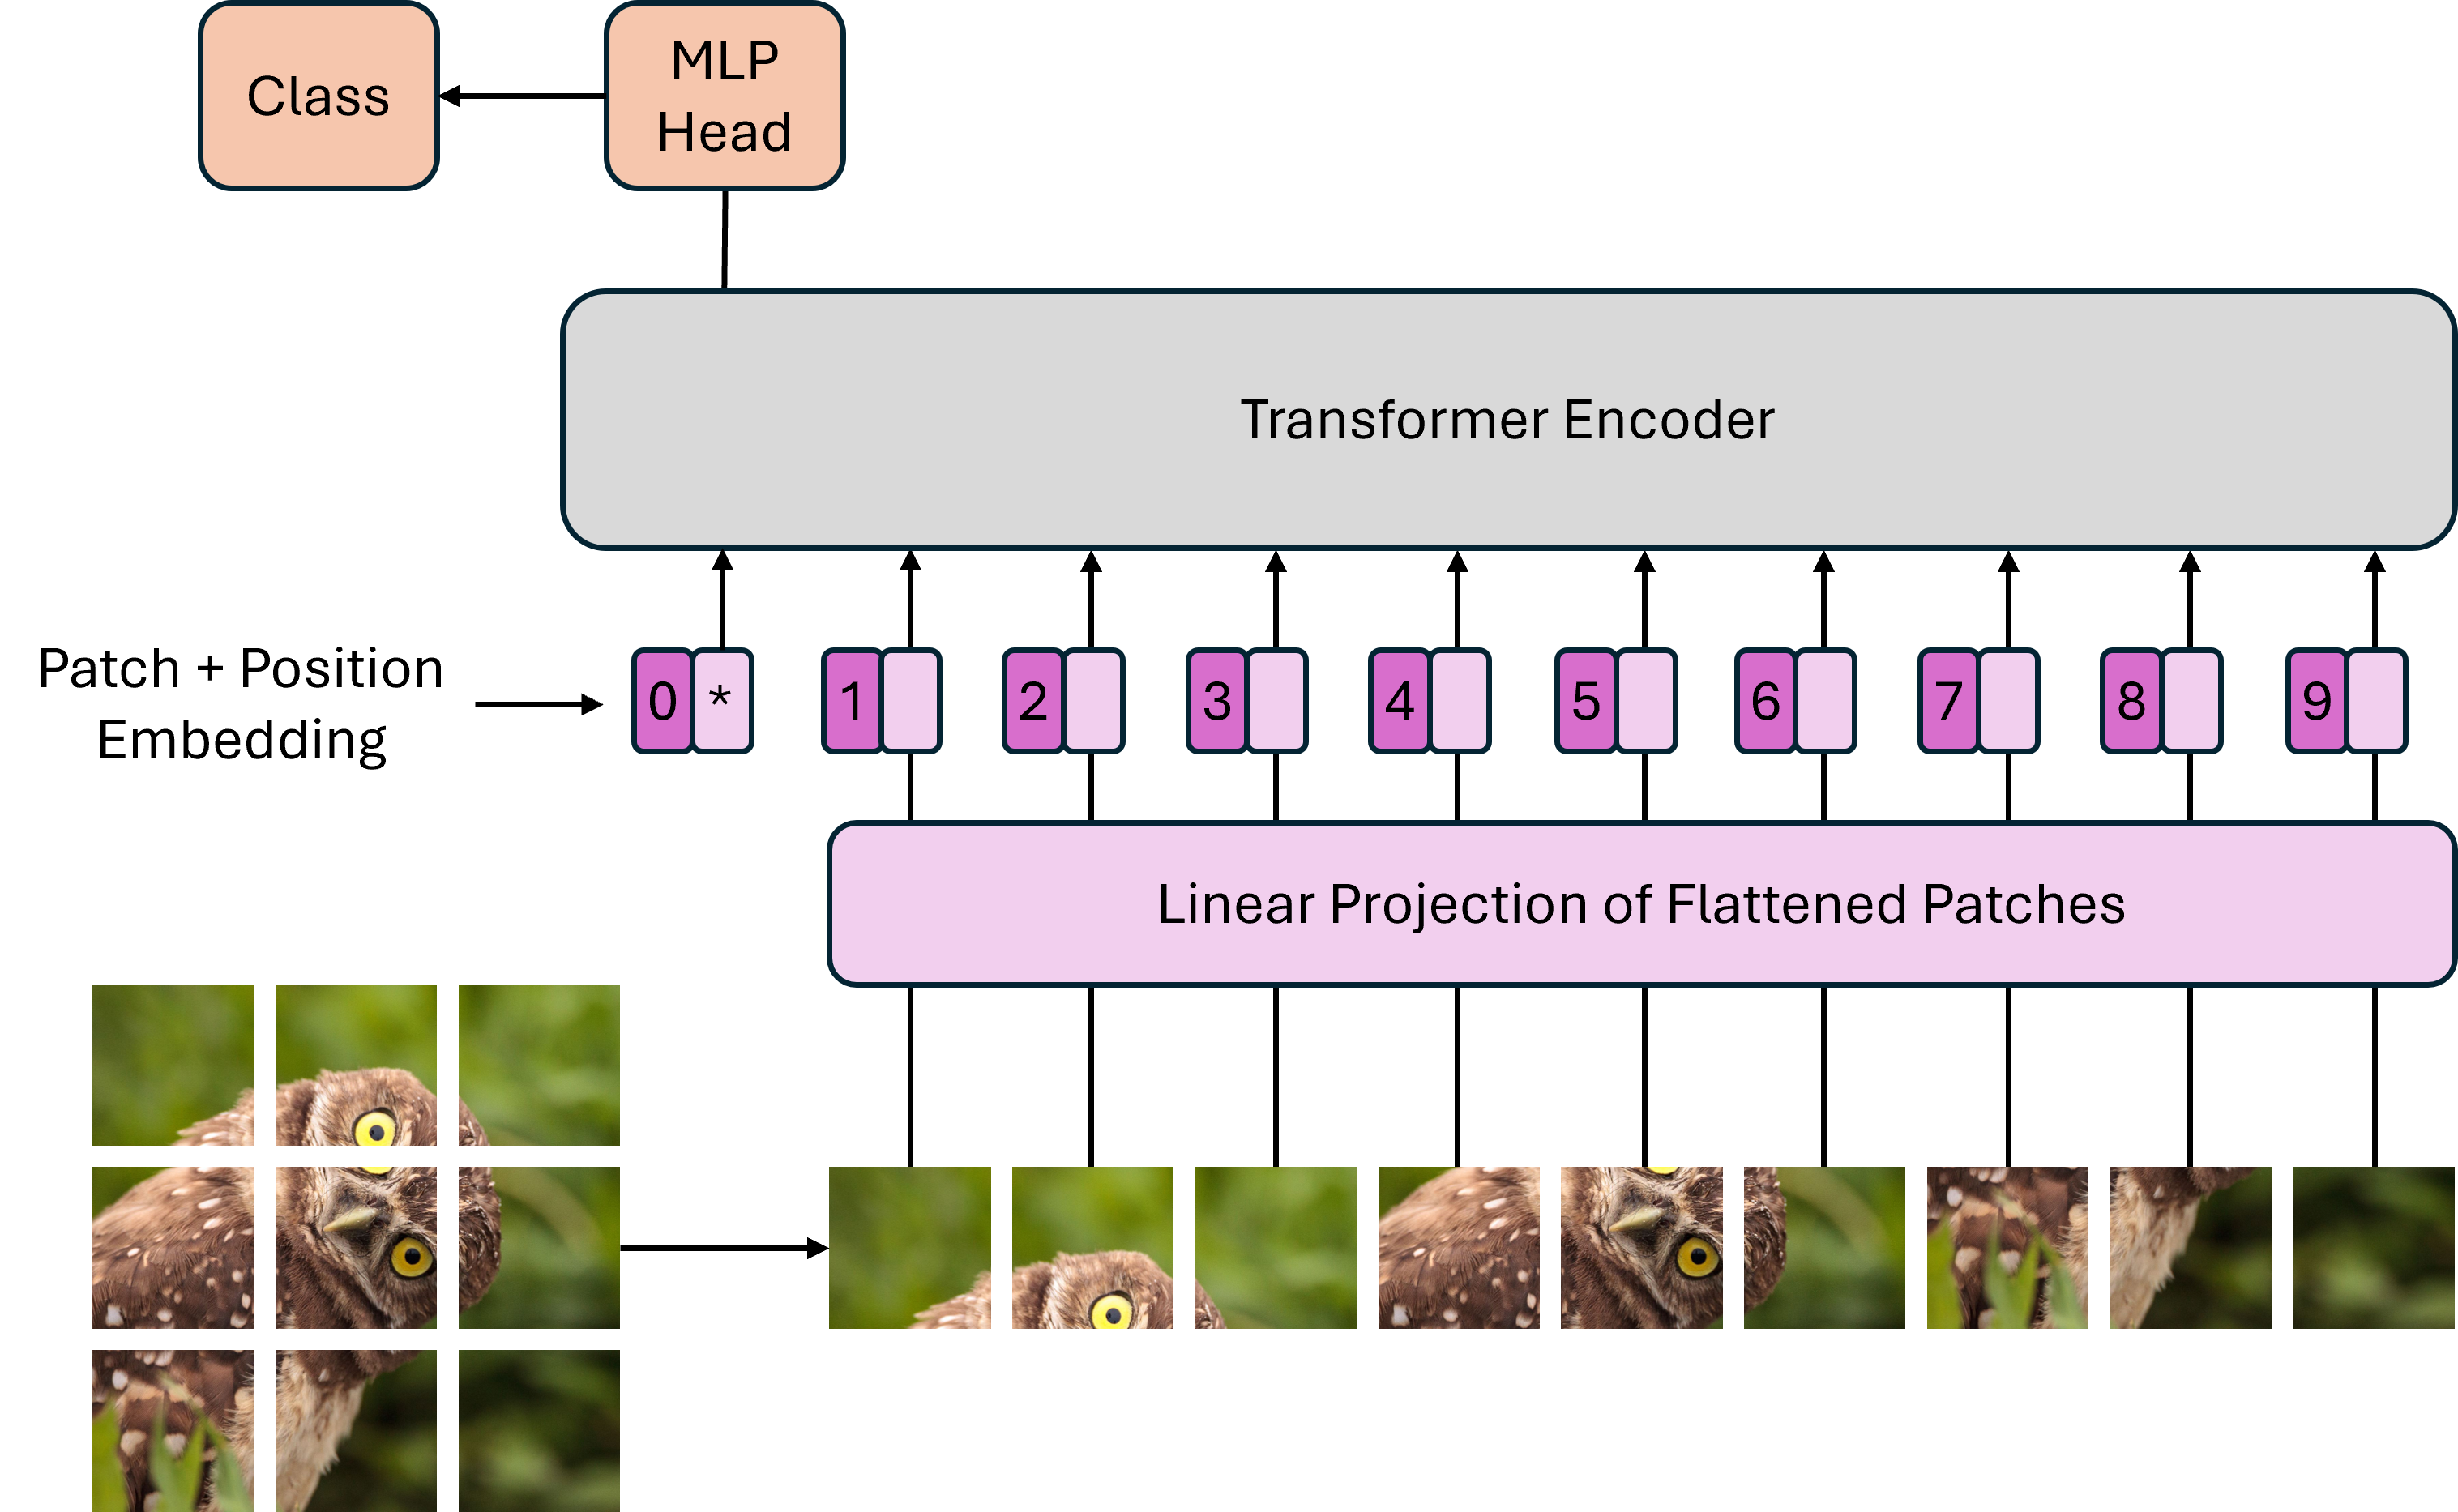
\includegraphics[width=0.75\textwidth]{pages/imgs/ViT.png}
	\caption{An illustration of the image tokenization process used in ViT. An image is split into fixed-size patches, which are then linearly projected and combined with positional embeddings to form a sequence of input vectors for the transformer encoder.}
	\label{fig:vit_diagram}
\end{figure}

\subsection{Contrastive Learning}
Contrastive learning, as the name suggests, is a training technique where contrastive data samples are evaluated against each other as a means of training a model to learn common and distinct attributes among samples of different classes (e.g., distinguishing a dog from a cat) \cite{contrastive_learning_multimodal_day}. In doing so, this technique tunes a model in such a way that allows it to encode embeddings where similar classes are close to one another in the embedding space, as opposed to distinct classes, which have a significant enough distance that allows the model to distinguish them.

More specifically, data samples are often partitioned into three distinct categories: (i) anchors, representing a base class for contrast, (ii) positives, with an equal class to that of the anchor, and (iii) negatives, representing a distinct class to that of the anchor.

On that note, an encoder is trained via contrastive learning such that embeddings of anchor and positive samples are close together, in the embedding space, as opposed to negative samples, which should be far apart. This is done so by tuning the encoder through a maximization or minimization of distance functions (e.g., Euclidean distance or cosine similarity) applied to the anchor and multiple positive samples, and the anchor and multiple negative samples, respectively, as illustrated in Figure~\ref{fig:contrastive_learning}, and described through the following formalisms:

\begin{enumerate}
  \item \textbf{Encoder and Embedding Definition:}
  Given an input sample \(I\) and an encoder \(\theta\), the latter produces a \(d\)‑dimensional embedding from the former:
  \begin{align}
      f = \theta(I) \;\in\;\mathbb{R}^d 
  \end{align}

  \item \textbf{Anchor, Positive, and Negative Samples Definition:}
    \begin{itemize}
      \item \emph{Anchor} \(I^a_i\), \(i=1,\dots,K\): Base samples;  
      \item \emph{Positive} \(I^+_i\), \(i=1,\dots,K\): Samples of the same class or augmented views of the anchors;
      \item \emph{Negative} \(I^-_j\), \(j=1,\dots,K\): Samples from different classes.
    \end{itemize}

  \item \textbf{Embedding Normalization:}
  For the proper application of a distance function, each embedding must be normalized to unit norm:
  \begin{align}
      \hat{f} = \frac{f}{\lVert f\rVert}
  \end{align}

  \item \textbf{Distance Function:}
  Compute the similarity measure via the distance function (cosine similarity is equivalent to the dot product):
  \begin{align}
      \delta(u, v) = u^\top v
  \end{align}

  \item \textbf{Contrastive Loss:}
    Provided an anchor \(I^a_i\), with a corresponding positive \(I^+_i\), and negatives \(\{I^-_{i,j}\}_{j=1}^K\), the loss for the anchor \(I^a_i\), where \(\tau>0\) is a temperature hyperparameter, is:
    \begin{align}
      \mathcal{L}_i = -\log
      \frac{\exp\bigl(\delta(\hat{f}_i, \hat{f}^+_i)/\tau\bigr)}
           {\exp\bigl(\delta(\hat{f}_i, \hat{f}^+_i)/\tau\bigr)
            + \sum_{j=1}^K \exp\bigl(\delta(\hat{f}_i, \hat{f}^-_{i,j})/\tau\bigr)}
    \end{align}

    \item \textbf{Overall Loss:}
    For a batch of \(N\) anchors, the overall loss is:
    \begin{align}
      \mathcal{L} = \frac{1}{N} \sum_{i=1}^N \mathcal{L}_i
    \end{align}
\end{enumerate}

\begin{figure}[h!]
	\centering
    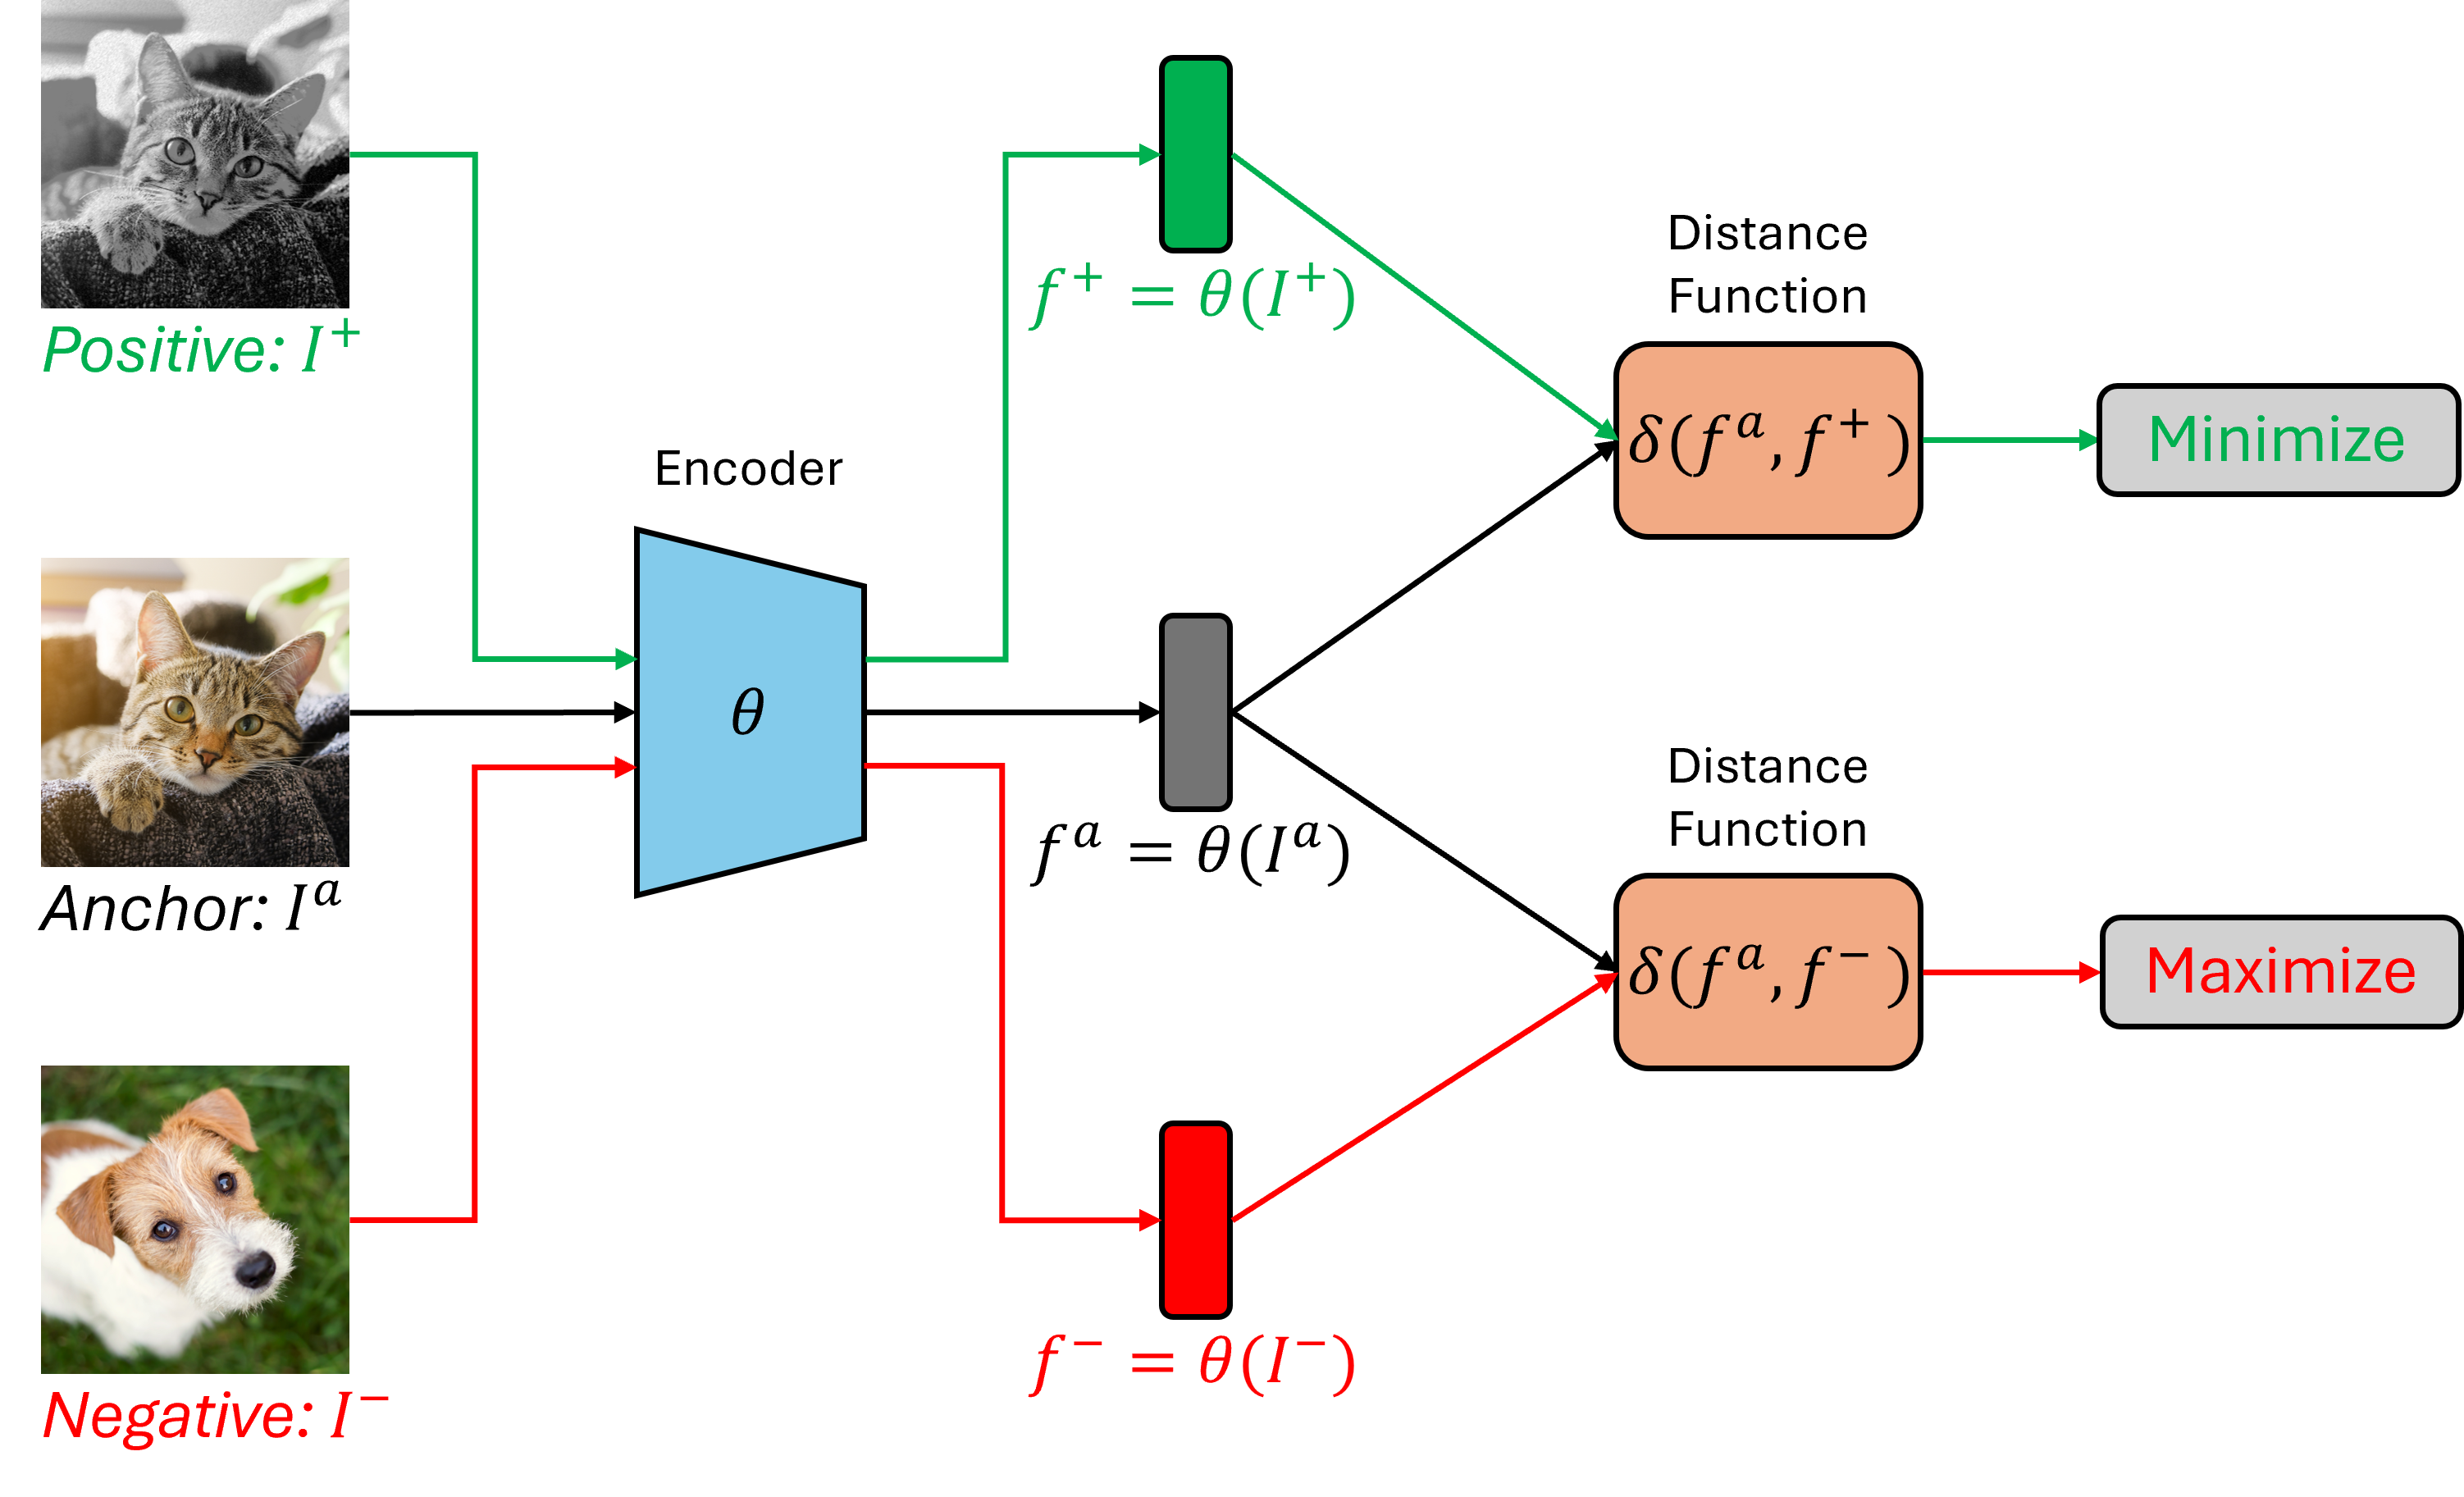
\includegraphics[width=0.75\textwidth]{pages/imgs/Contrastive_Learning.png}
	\caption{A high-level illustration of the contrastive learning framework, where an encoder is trained to minimize and maximize the distance function between an anchor and its contrastive positive and negative samples, respectively. Here, the positive sample is a transformation of the original image.}
	\label{fig:contrastive_learning}
\end{figure}

Finally, it is worth mentioning the role of data augmentation in such frameworks. Positive samples are either images containing data that fits within the same class as the anchor or augmentations of the anchor (i.e., multiple patches and transformations), ranging from color jittering and rotation to noise injection and random affine transformations. This is done to ensure that the model does not conform to unwanted patterns (e.g., pixel-level or rotation-specific artifacts), but instead learns the core features that characterize these classes (e.g., shapes, contours, textures, and spatial configurations), which in turn allows for proper generalization. After training, the resulting encoder should be capable of accurately distinguishing between similar and dissimilar classes, as illustrated in Figure~\ref{fig:contrastive_learning_embedding_space}.

\begin{figure}[h!]
	\centering
    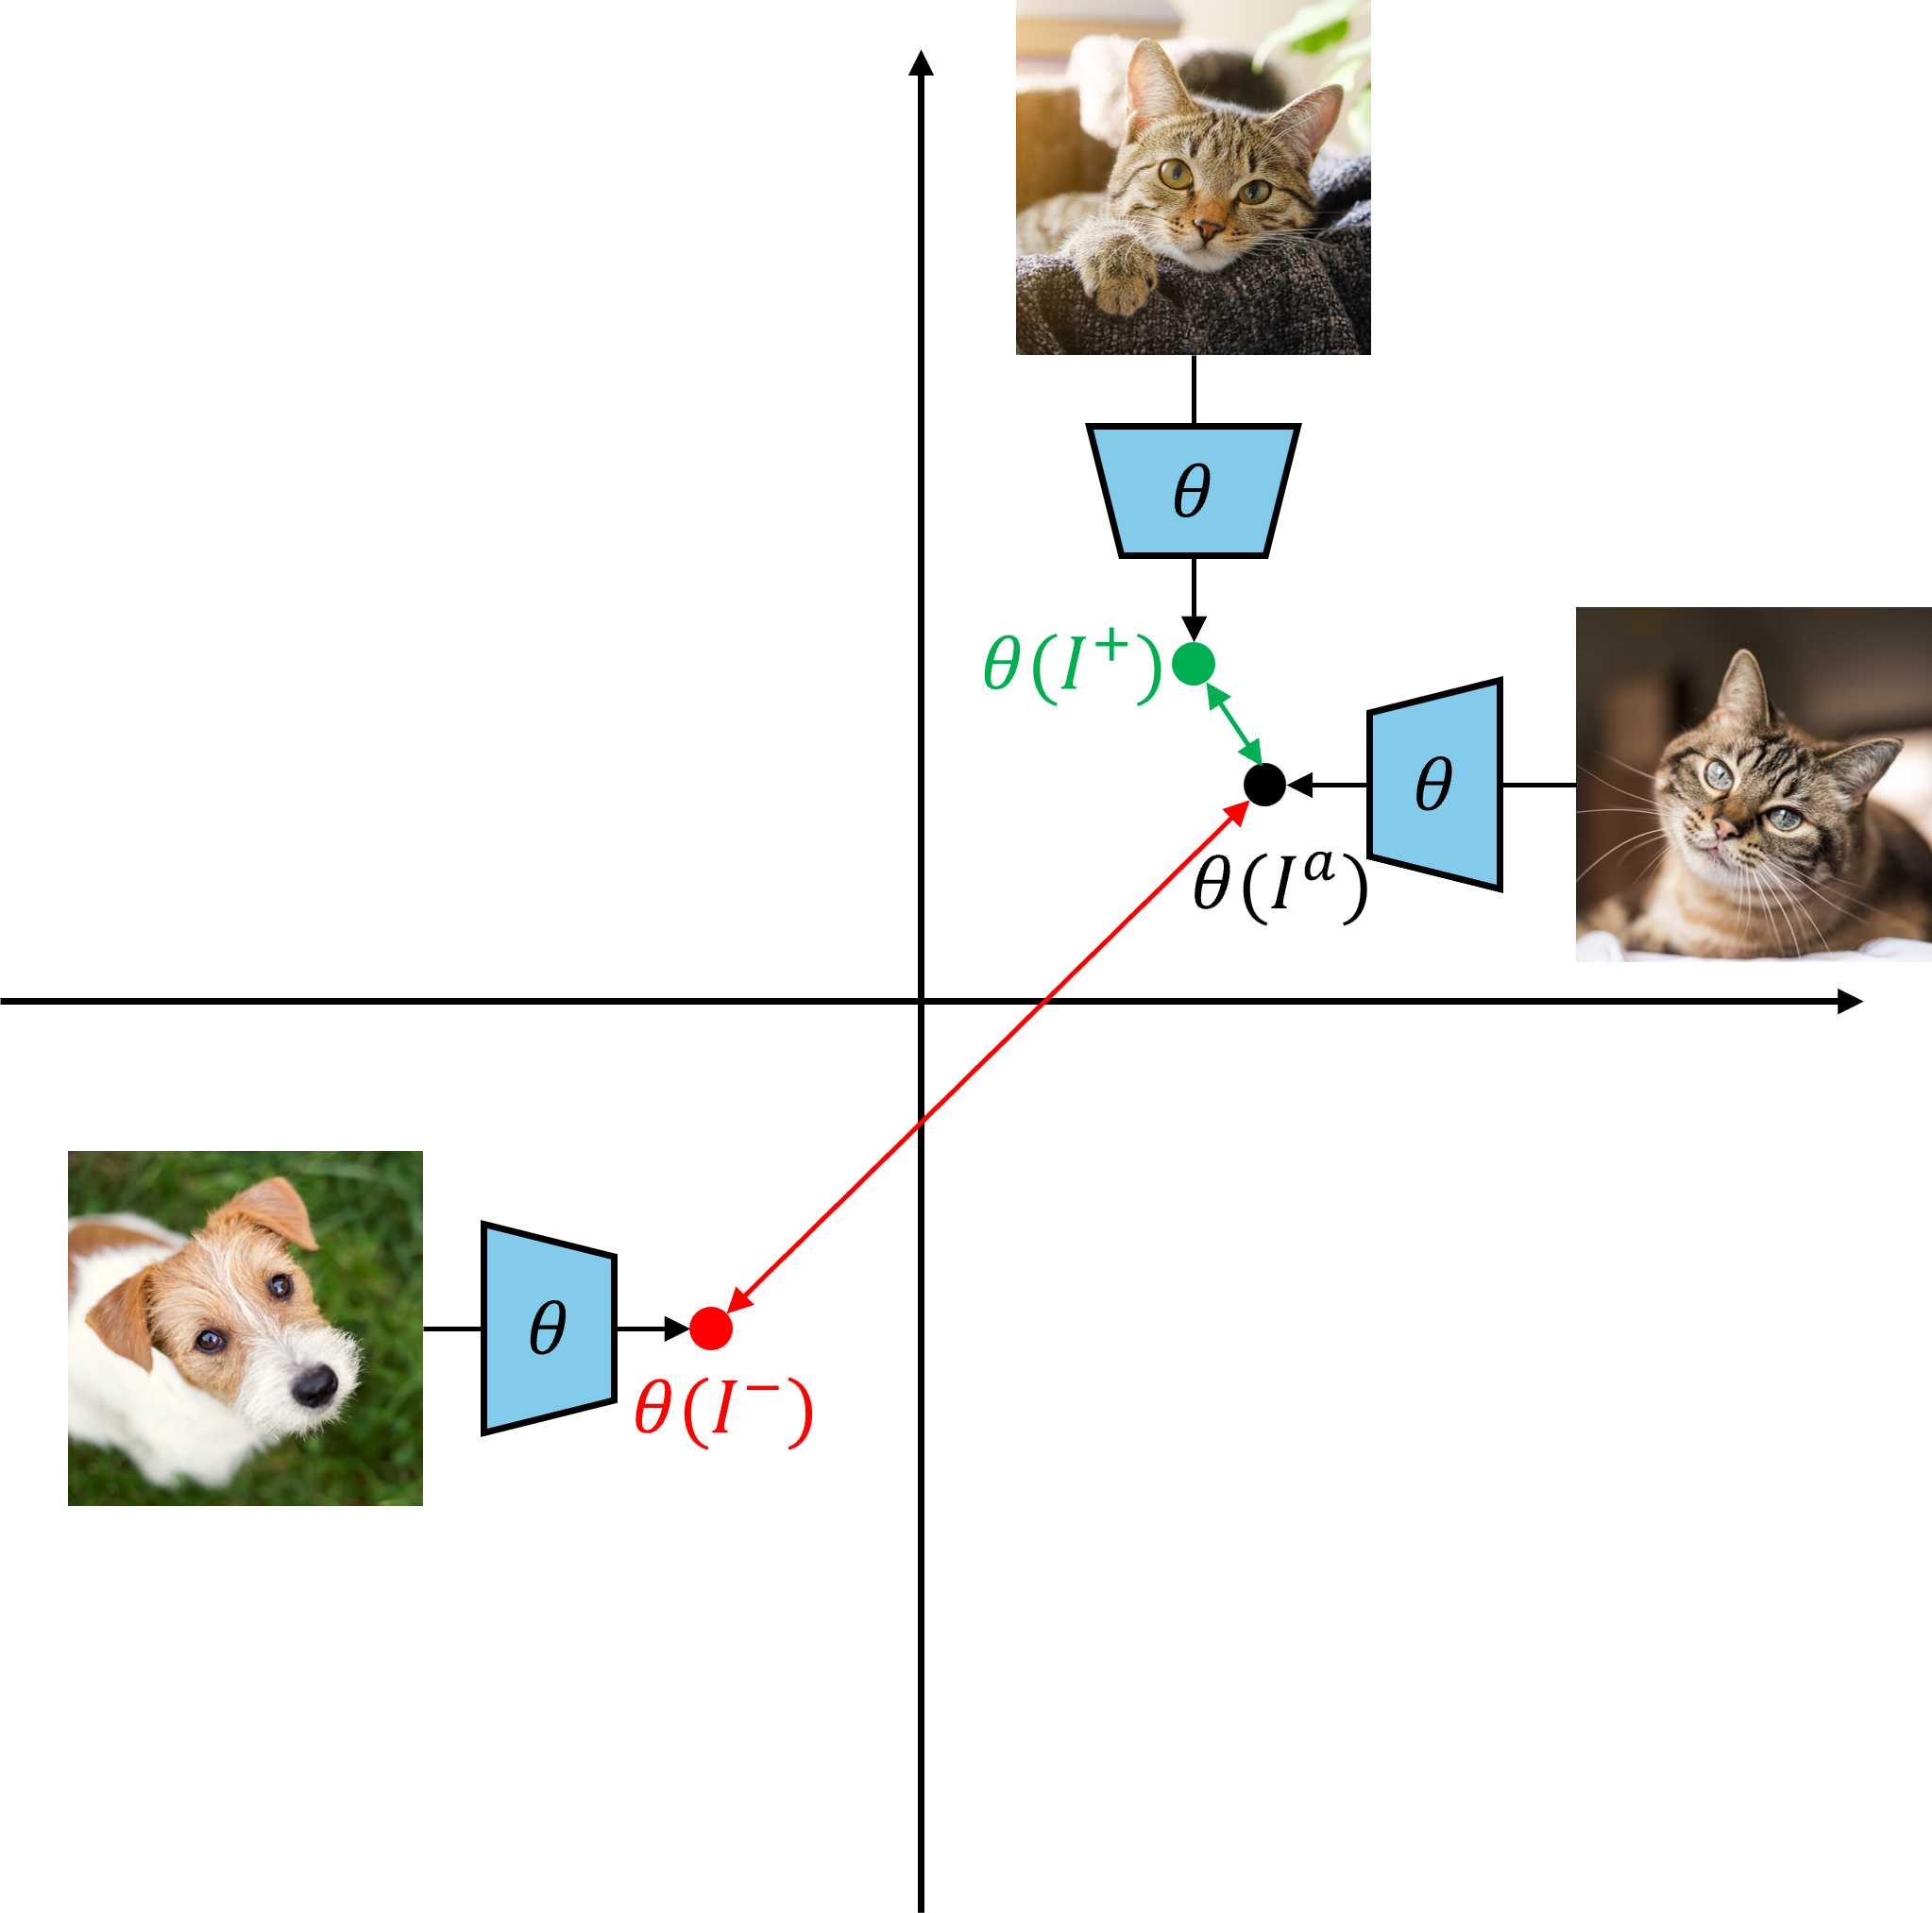
\includegraphics[width=0.55\textwidth]{pages/imgs/Contrastive_Learning_Embedding_Space.png}
	\caption{An illustration of the embedding space of a properly tuned encoder that sets distinct classes far apart, while shortening the distance of similar samples as per contrastive learning. Here, the black data point serves as the anchor, the green data point as the positive sample, and the red data point as the negative sample. Note the difference in distance from the anchor to the positive and negative samples.}
	\label{fig:contrastive_learning_embedding_space}
\end{figure}

\section{Multimodal Architectures}
The core building block of modern multimodal systems often involves combining powerful pre-trained unimodal models. Unlike standard Transformers, which operate on a single sequence of tokens, multimodal models must compare fundamentally different data structures (e.g., image patches and text tokens). The solution is to create a ``common language'' known as the shared embedding space. This is a high-dimensional vector space where both images and text can be represented. As such, the goal is to train encoders that map semantically similar image-text pairs close to each other in this space. There are three main approaches:
\begin{enumerate}
\item \textbf{Dual Encoders:} This architecture, popularized by CLIP, uses two separate encoders—one for each modality (a ViT for images and a standard Transformer for language). The encoders are trained jointly with the contrastive learning to align their output embedding spaces. This design is highly efficient for retrieval tasks.

\item \textbf{Fusion Encoders:} These models use a single Transformer encoder that processes the combined inputs from multiple modalities. This enables ``cross-attention'' between image patches and text tokens at a much deeper level, allowing for more complex reasoning. Models like ViLT and VisualBERT follow this pattern.

\item \textbf{Encoder-Decoders:} These models are used for generative tasks. An encoder processes one modality (e.g., an image), and a decoder uses that representation to generate output in another modality (e.g., a text caption). Models like BLIP and Flamingo are powerful examples used for image captioning and visual question answering.
\end{enumerate}
\noindent Even though these models are used for different purposes, their architectures are very similar. Today's exercises, however, will focus on the dual encoder architecture, as it provides the clearest illustration of cross-modal alignment.

\subsection{CLIP:}
\label{subsec:clip_stuff}
%As previously detailed, CLIP resorts to a dual encoder architecture to encode images and text in a shared embedding space through a ViT and a standard Transformer, respectively \cite{clip_multimodal_day}. The idea is to train this model---via contrastive learning---in such a way that maximizes the similarity of the encoded image-text pairs, while minimizing the similarity of disparate encoded image-text pairs (i.e., the embedding of the sentence ``a gray british shorthair cat'' should be similar to the embedding of an image of a cat, as opposed to that of a dog). In doing so, such allows the establishment of relationships between image-text pairs that serve a myriad of purposes, ranging from image classification to more sophisticated integrations in generative scenarios. One interesting aspect about CLIP is its capability of generalizing to tasks it was not trained on (i.e., zero-shot classification)---a surprising example being CLIP's performance matching the accuracy-level of the famous ResNet-50 without actually training on the data which ResNet-50 trained on.

%More specifically, focusing on the base case for image classification, CLIP takes a given number of text embeddings, via a standard Transformer---usually text labels scraped from large datasets of image captions from the web---, followed by multiple image embeddings, via a ViT, matching each of the previous labels. Next, the dot product (i.e., cosine similarity) is applied to each possible image-text embedding pair. Thus, the model is iteratively trained in such a way that matching image-text embeddings stay close together in the embedding space and dissimilar pairs far apart, as per contrastive learning, as illustrated in Figure~\ref{fig:clip_contrastive_pre_training}.

As previously detailed, the Contrastive Language-Image Pre-training (CLIP) model employs a dual-encoder architecture to encode images and text into a shared embedding space, utilizing a Vision Transformer (ViT) for images and a standard text Transformer for text \citep{clip_multimodal_day}. The core idea is to train this system via contrastive learning on a massive dataset of image-text pairs. This process is designed to maximize the similarity of correctly paired image and text embeddings while simultaneously minimizing the similarity of disparate pairs. For instance, the embedding of the sentence ``a gray British shorthair cat'' should be mathematically close to the embedding of an image of that cat, but distant from the embedding of a picture of a dog. More specifically, focusing on the base case for image classification, the model takes a given number of text embeddings -- usually derived from descriptive captions -- and a corresponding set of image embeddings. Next, the dot product, which represents the cosine similarity, is calculated for every possible image-text embedding pair. The model is then iteratively trained to ensure that the similarity score for matching image-text embeddings is high, pulling them closer together in the embedding space. At the same time, the score for dissimilar pairs is low, causing them to be pushed far apart. This direct application of contrastive learning is illustrated in Figure~\ref{fig:clip_contrastive_pre_training}.

The true power of this methodology is revealed in CLIP's groundbreaking capability for zero-shot classification. This allows the model to accurately classify images from categories it was never explicitly trained to recognize, establishing relationships that serve a myriad of purposes, from basic classification to sophisticated integrations in generative scenarios. Instead of relying on a predefined label, it dynamically classifies an image by finding the best match between the image's embedding and the text embeddings of potential descriptions. A surprising and powerful example of this is CLIP's ability to match the accuracy level of the famous ResNet-50 on the ImageNet benchmark, crucially, without having been trained on the specific labeled dataset that ResNet-50 was trained on.

\begin{figure}[h!]
	\centering
    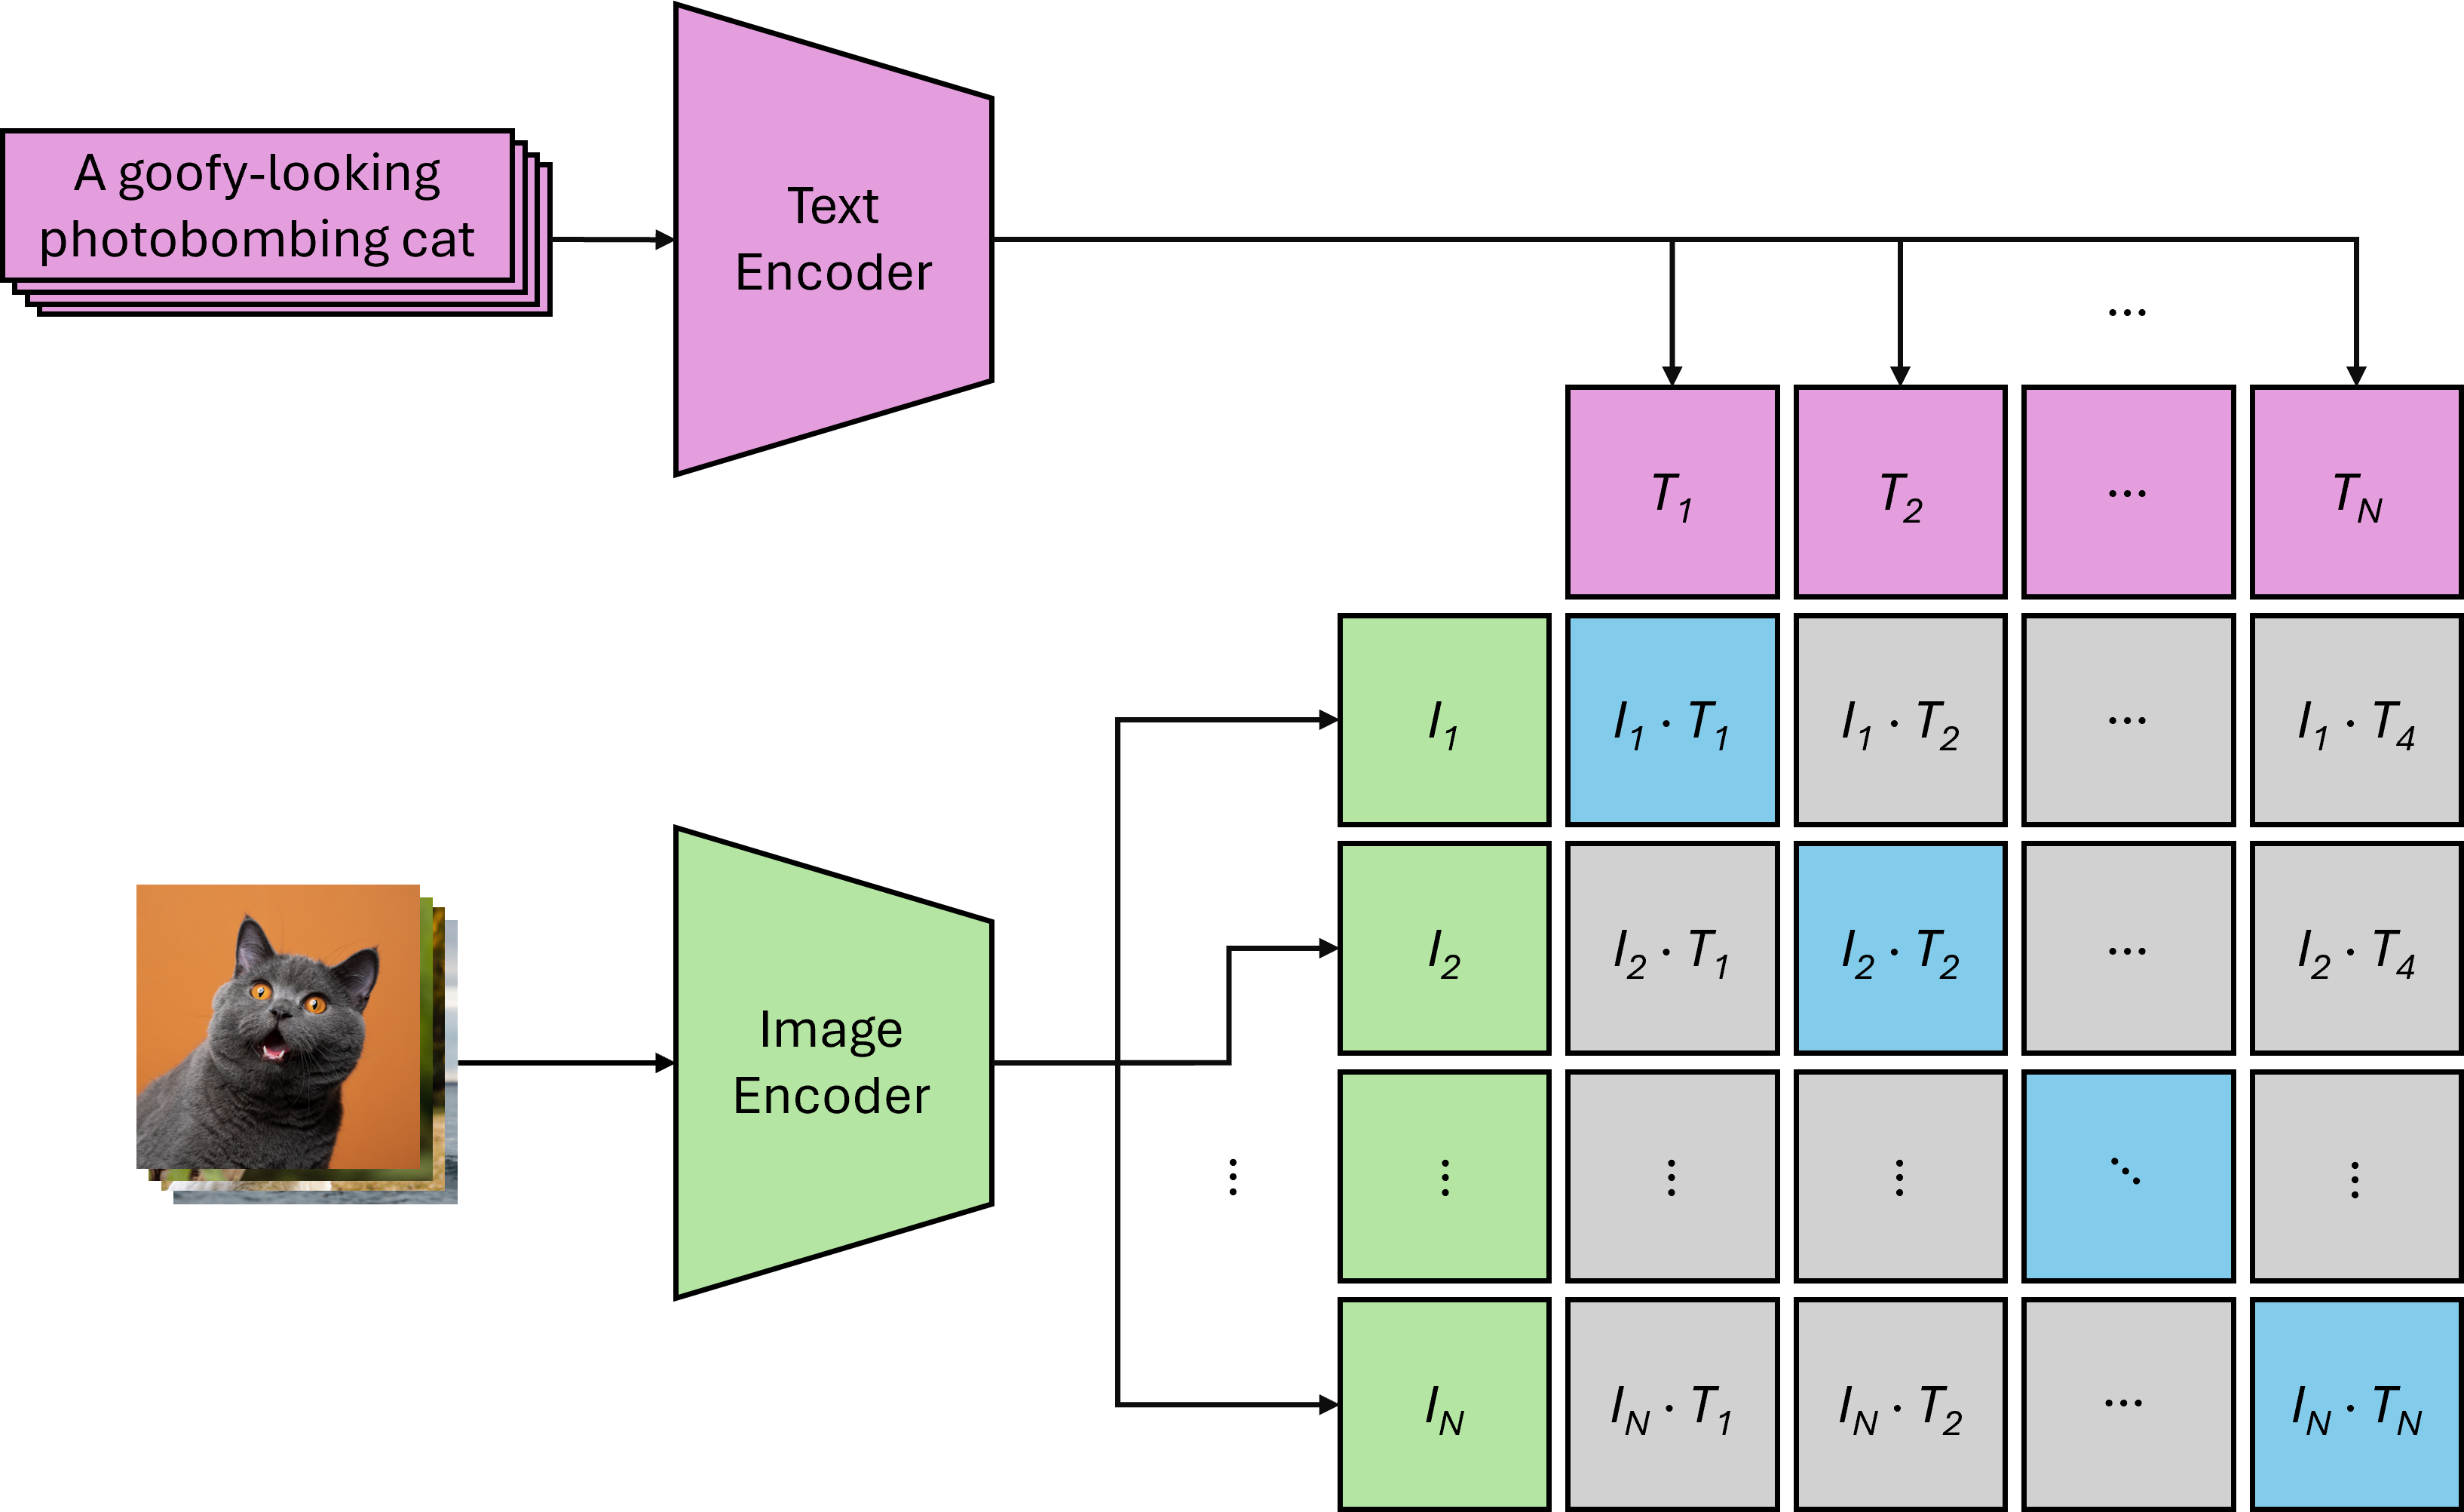
\includegraphics[width=0.75\textwidth]{pages/imgs/CLIP_Contrastive_Pre_Training.png}
	\caption{An illustration of CLIP's dual encoder architecture. Images and texts are embedded and individually paired with one another via a distance function to rank for similarity. The model is then iteratively tuned to achieve proper distance values and enable accurate classification (the values of the matrix's diagonal should be minimized and the remaining cells maximized).}
	\label{fig:clip_contrastive_pre_training}
\end{figure}

This last step is done symmetrically---by performing a loss through both ways (i.e., text-to-image and image-to-text), which is later averaged into one component---to ensure proper alignment between both modalities. Since CLIP learns broad vision–language alignments from large-scale web data, it can be applied in zero-shot fashion to downstream tasks without further fine-tuning, simply by filling out a default prompt of the form ``a photo of a \{class\}'', where '\{class\}' is replaced by the label whose text embedding is most similar to the embedding of the image (see Figure~\ref{fig:clip_zero_shot}).

Formally speaking, CLIP uses a dual‑encoder architecture to map images and text into a shared \(d\)‑dimensional embedding space, and trains via a symmetric contrastive objective as per the following formalisms:

\begin{enumerate}
  \item \textbf{Encoders and Embeddings Definition:}
  Given an image domain \(I\) and a text domain \(T\), where \(f_i = \theta(I_i)\) and \(g_i = \phi(T_i)\), we have:
  \begin{align}
      \theta : I \to \mathbb{R}^d,\quad
      \phi : T \to \mathbb{R}^d
  \end{align}

  \item \textbf{Embedding Normalization:}
  Each embedding must be normalized to unit form for proper application of the distance function:
  \begin{align}\label{eq:embedding_normalization}
      \hat f_i = \frac{f_i}{\lVert f_i\rVert},\quad
      \hat g_i = \frac{g_i}{\lVert g_i\rVert}
  \end{align}

  \item \textbf{Distance Function:}
    Compute the distance between each image-text embedding pair via cosine similarity:
    \begin{align}\label{eq:cosine_similarity}
      \delta_{ij} = \hat f_i \cdot \hat g_j
    \end{align}

  \item \textbf{Symmetric Contrastive Loss:}
    For a batch of \(N\) matched image-text pairs \((I_i,T_i)\), we have a loss function for each direction (i.e., image-to-text and text-to-image), together with the total loss:
    \begin{align}
      \mathcal{L}_{\mathrm{I2T}} = -\frac{1}{N}\sum_{i=1}^N
      \log\frac{\exp(\delta_{ii})}{\sum_{j=1}^N \exp(\delta_{ij})},
    \end{align}
    \begin{align}
      \mathcal{L}_{\mathrm{T2I}} = -\frac{1}{N}\sum_{j=1}^N
      \log\frac{\exp(\delta_{jj})}{\sum_{i=1}^N \exp(\delta_{ij})},
    \end{align}
    \begin{align}
      \mathcal{L} = \frac{1}{2}\bigl(\mathcal{L}_{\mathrm{I2T}} + \mathcal{L}_{\mathrm{T2I}}\bigr)
    \end{align}

  \item \textbf{Zero‑Shot Classification:}
    Given an image \(I\) and a set of \(K\) candidate class names \(c_k\), form prompts
    \(\,T_k = \text{“A photo of a }c_k\text{”}\), normalize each prompt to unit norm, and compute the probability of class \(k\) matching image \(I\):
    \begin{align}
      p(y=k\mid I) = \frac{\exp\bigl(\hat f\cdot \hat g_k)}{\sum_{j=1}^K \exp\bigl(\hat f\cdot \hat g_j)}
    \end{align}
\end{enumerate}

\begin{figure}[h!]
	\centering
    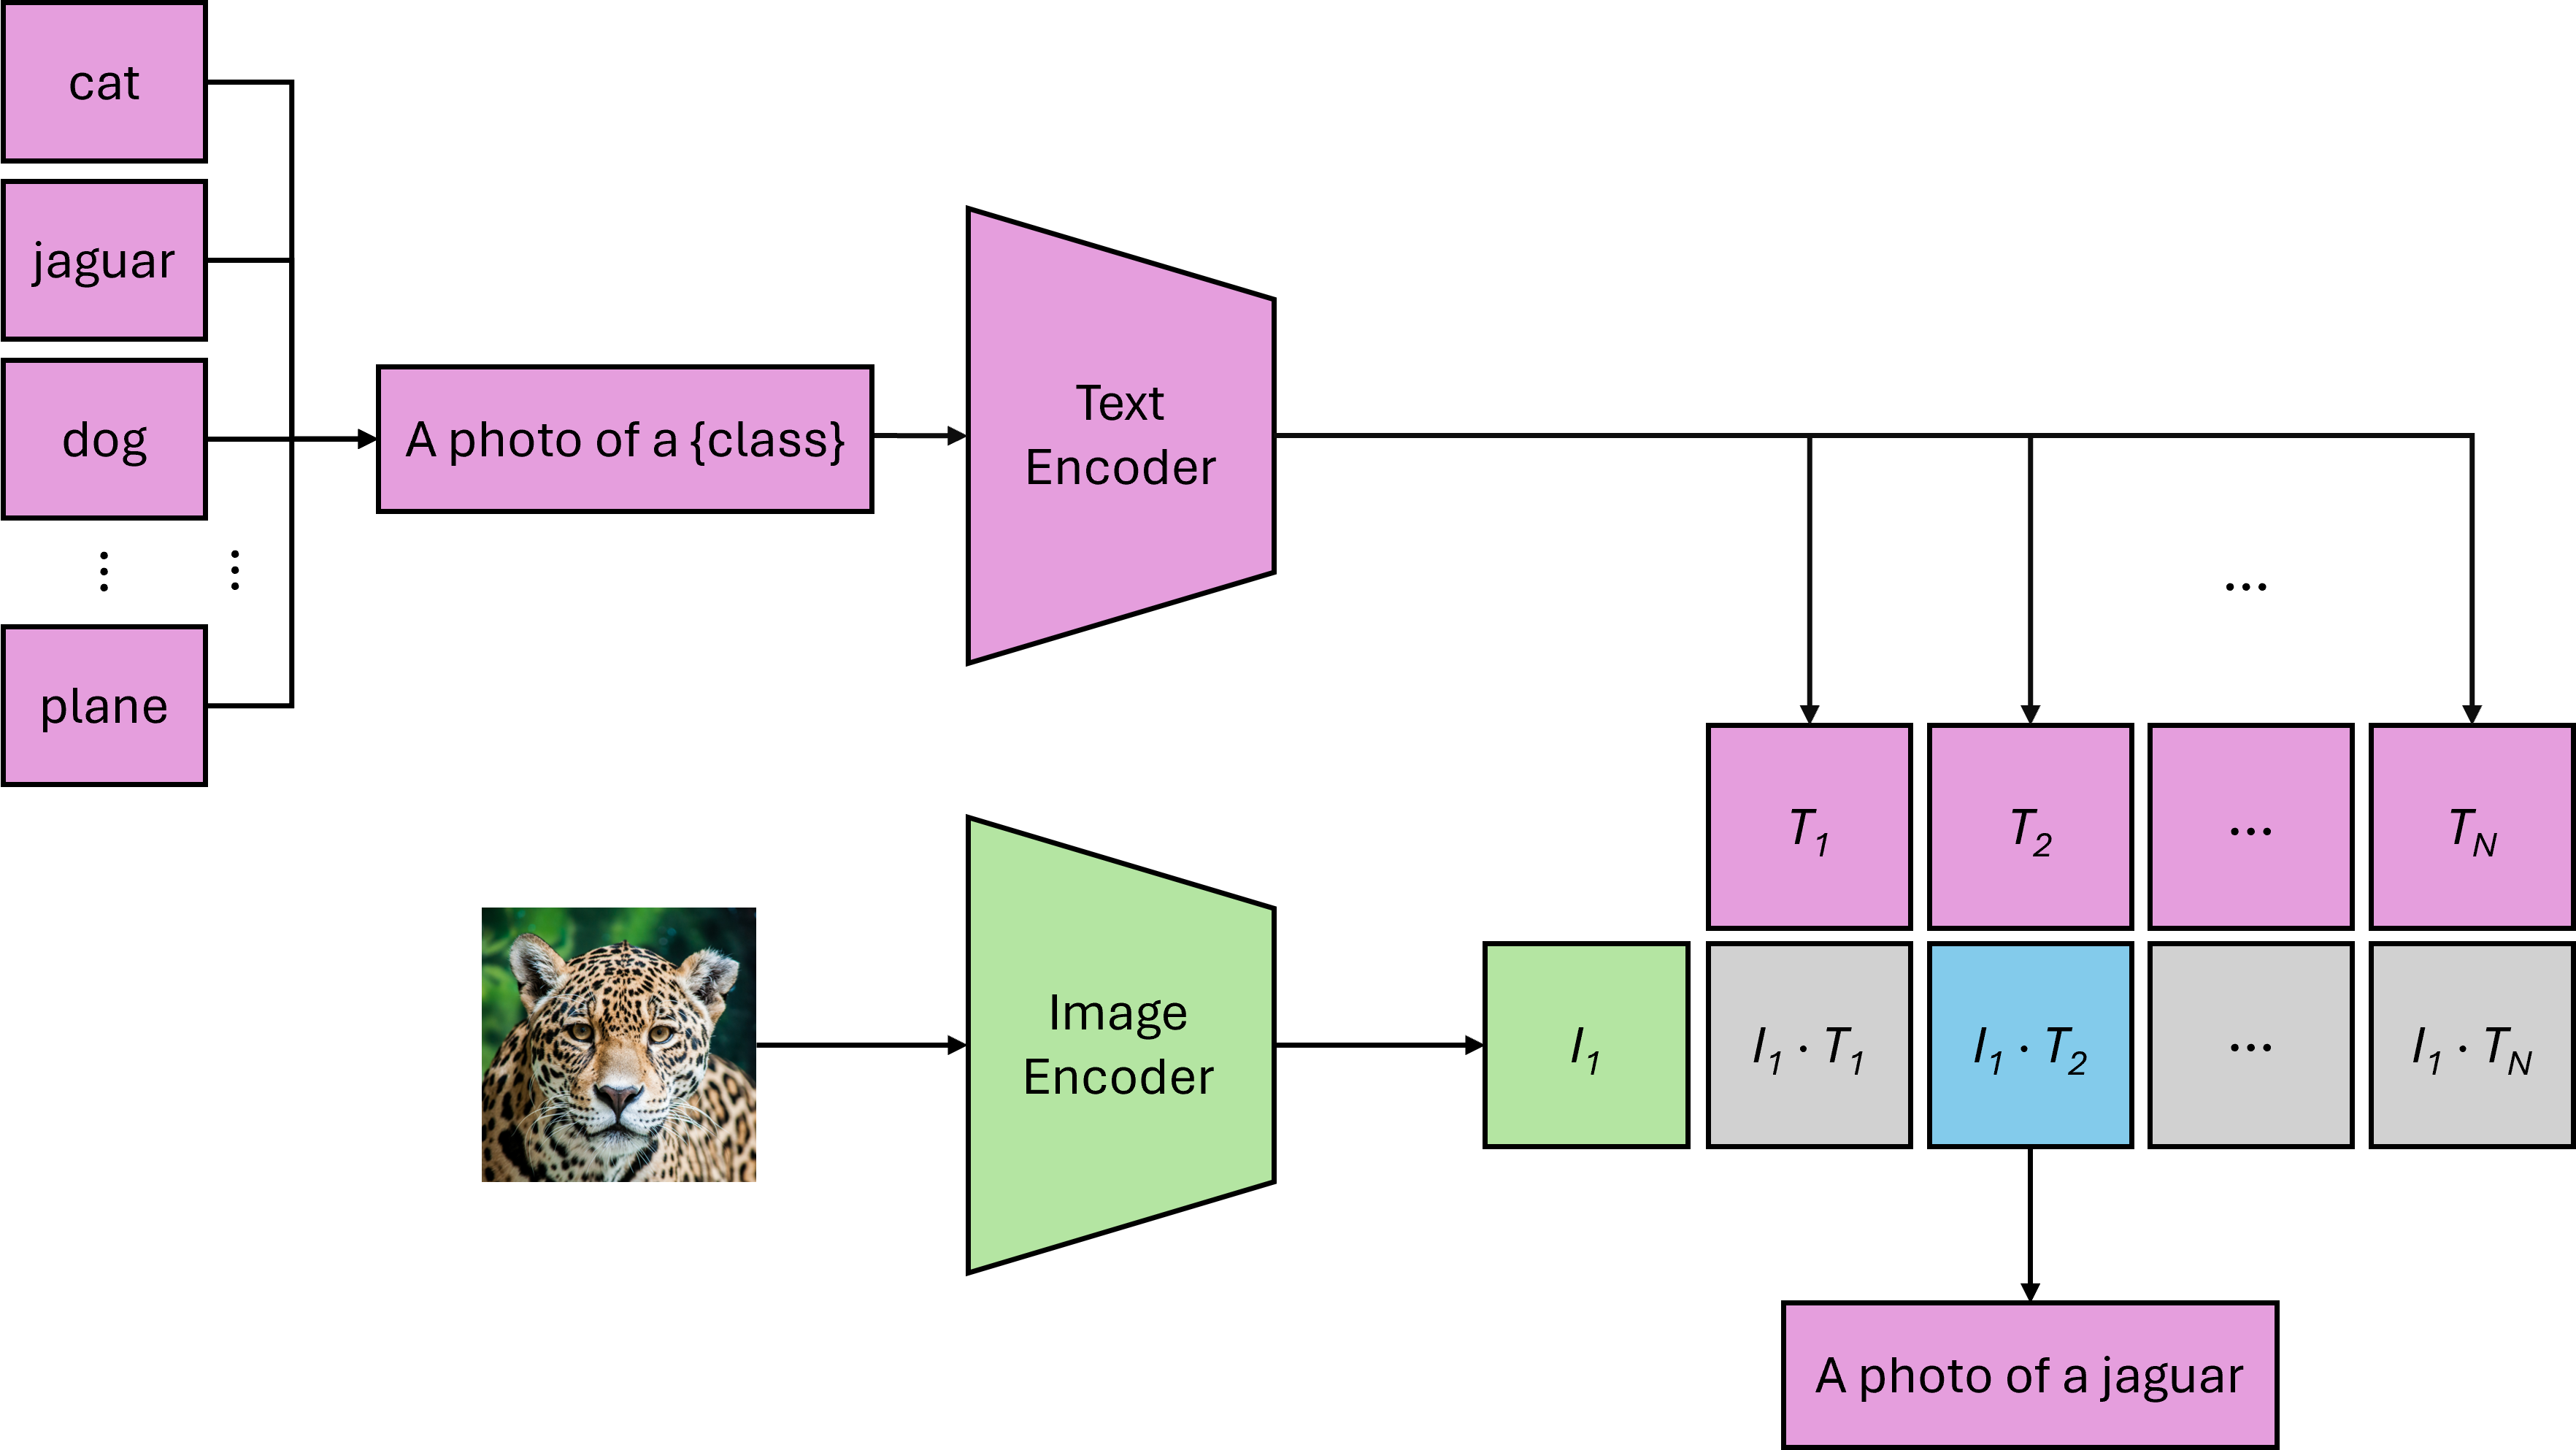
\includegraphics[width=0.75\textwidth]{pages/imgs/CLIP_Zero_Shot.png}
	\caption{An illustration of CLIP's zero-shot classification. After training, CLIP is capable of properly classifying an image provided the properly tuned weights that result from the pre-training. Similarity measures are computed between the image and each possible text pair and the shortest distance denotes the right class.}
	\label{fig:clip_zero_shot}
\end{figure}

\begin{exercise}
Let us now apply the previous principles in practice. You will implement multiple functions, each serving a different purpose, covering the processing, embedding, and classification of image-text pairs. In essence, you will be feeding a ViT and a standard Transformer with the intended data, which will enable image-text pair classification using CLIP's approach. To that end, this exercise will guide you through the completion of the corresponding yet-to-be-completed notebook cells present in \texttt{lxmls/labs/notebooks/multimodal/clip\_exercise.ipynb}:

\begin{enumerate}
    \item \textbf{Basic setup:} Run the first two cells of the notebook to import all necessary dependencies for proper execution of all code cells.

    \item \textbf{Data and model setup:} Run all subsequent cells until Cell 19 (inclusive). This will enable you to execute the following steps automatically:
    \begin{itemize}
        \item Prepare the ViT's input (i.e., loading an example image of two cats);

        \item Initialize the GPT model from the previous day for image labelling;

        \item Prepare a string to use as a default for image classification (this will later append individual GPT-generated labels);

        \item Load and prepare a CLIP model;

        \item Convert the example image using the image processor;

        \item Load a tokenizer and tokenize the previously defined image labels;

        \item Embed the image labels and visualize the outcome of splitting the example image into fixed size patches;

        \item Store the learned weights for linearly projecting the image.
    \end{itemize}

    \item \textbf{Prepare the image for projection to the embedding space:} You will now implement a function whose purpose is to project the image, in its entirety, to the embedding space. For that to happen, define the following steps in sequence:
    \begin{itemize}
        \item Break the image into multiple patches of fixed size (patch\_size, patch\_size) (Hint: Take a peek at Cell 18. How can we declare patches?);

        \item Apply a learnable linear layer to each patch (Hint: Take a peek at Cell 19 and Eq.~\ref{eq:linear_projection});

        \item Assign each linearly projected patch embedding to the \texttt{manual\_patch\_embeds} variable.
    \end{itemize}
    \begin{python}
def get_patch_embeddings(pixel_values, filter_weights):
"""using a similar code as the visualization above, project the image patches in the embedding space"""
    assert len(pixel_values) == 1 # we do it for a single image for the example
    manual_patch_embeds = torch.zeros(num_patches, num_patches, filter_weights.shape[0], device=model.device)
    
    # YOUR SOLUTION HERE
    
    return manual_patch_embeds
    \end{python}

    \item \textbf{Flatten the embeddings and check for correctness:} Run all subsequent cells until Cell 22 (inclusive). This will enable you to automatically execute the following steps:
    \begin{itemize}
        \item Retrieve the linearly projected patch embeddings, as per the function you've just defined, and flatten it (notice the difference in shape before and after flattening);

        \item Compare your results with the original implementation to assure correctness (this will allow you to test if you implemented the previous function as intended).
    \end{itemize}

    \item \textbf{Prepare the class token and positional embeddings:} You will now implement a function that serves the following purposes:
    \begin{itemize}
        \item Prepend a learnable class embedding to the previously defined patch embeddings (already implemented for convenience)

        \item Add a learnable positional embedding to retain information about each patch's location in the original image (Hint: Take a peek at Eq.~\ref{eq:class_token_positional_embeddings}, look through the possible method calls of the model, and respective arguments)
    \end{itemize}
    \begin{python}
def get_add_cls_and_position(manual_patch_embeds):
    """The only thing left to do is to add class and position embedding"""
    class_embeds = model.vision_model.embeddings.class_embedding.expand(batch_size, 1, -1)
    hidden_states = torch.cat([class_embeds, manual_patch_embeds], dim=1)
    
    # YOUR SOLUTION HERE
    
    hidden_states = model.vision_model.pre_layrnorm(hidden_states)
    return hidden_states
    \end{python}

    \item \textbf{Conclude the image embedding and project the image-text pairs:} Run all subsequent cells until Cell 27 (inclusive). This will enable you to automatically execute the following steps:
    \begin{itemize}
        \item Retrieve the class and positional embeddings in conjunction with the patch embeddings;

        \item Feed the previously declared embeddings to the ViT;

        \item Extract the class token representation;
        
        \item Apply the final normalization to obtain the image embedding;

        \item Project both the text and image embeddings to the shared embedding space (see Figure~\ref{fig:clip_contrastive_pre_training} for a visual explanation)
    \end{itemize}

    \item \textbf{Define the distance function:} You will now implement a function whose purpose is extracting the similarities between all image-text embedding pairs. To accomplish that, define the following steps in sequence:
    \begin{itemize}
        \item Normalize each embedding (Hint: Take a peek at Eq.~\ref{eq:embedding_normalization});

        \item Apply the cosine similarity to the embeddings (Hint: Take a peek at Eq.~\ref{eq:cosine_similarity})
    \end{itemize}
    \begin{python}
def get_sim(text_embedding, image_embedding):

    # YOUR SOLUTION HERE
    
    return similarities
    \end{python}

    \item \textbf{Retrieve the similarities:} Run Cell 29 to retrieve the similarities as per the function you've just defined.

    \item \textbf{Define a rerank function:} You will now implement a function whose purpose is reranking the retrieved similarities between all image-text embedding pairs, in descending order, such that the class with highest probability stays on top:
    \begin{python}
def rerank(similarities):
    """All is left to do is sort the similarities to rerank the text"""
    
    # YOUR SOLUTION HERE

    return ranking
    \end{python}

    \item \textbf{Analyze the results:} Run all remaining cells. This will enable you to automatically execute the following steps:
    \begin{itemize}
        \item Apply the reranking function to the similarity scores;

        \item Print the resulting similarities in descending order, guaranteeing that the classification with the highest probability stays on top (see Figure~\ref{fig:clip_zero_shot} for a visual description).
    \end{itemize}
    What can you conclude by analyzing the results? Does your implementation work as intended?
\end{enumerate}
\end{exercise}

%\section{From Self-Attention to Cross-Modal Alignment}
%In Transformers, \textbf{self-attention} calculates the relationships between all pairs of tokens within a single sequence. A token effectively asks, ``Which other tokens in \textit{this sentence} are most important to understanding my meaning?'' (see Figure \ref{fig:attention_comparison}).

%\textbf{Cross-modal alignment} extends this idea. A text embedding asks, ``Which image embedding in \textit{this batch} is most similar to my meaning?'' or an image embedding asks, ``Which text description best represents \textit{me}?'' This shift from intra-sequence relationships to inter-modality similarity is the key conceptual leap. Instead of attending to nearby words, the model attends to concepts across a representational space.

%\begin{figure}[h!]
	%\centering
    % TODO: Create Figure
    %\includegraphics{path/to/image.png}[width=0.9\textwidth]
	%\caption{On the left, a standard self-attention mechanism where a token ("it") attends to other tokens ("the cat") within the same sentence. On the right, a simplified view of cross-modal alignment, where an image embedding is pulled closer to its correct text description ("a photo of a cat") and pushed away from incorrect ones in a shared embedding space.}
	%\label{fig:attention_comparison}
%\end{figure}

%\begin{exercise}
%Zero-Shot Image Classification with CLIP

%Let's implement the core logic of a CLIP-powered system. We will perform zero-shot classification by calculating the similarity between a single image and multiple text descriptions.
%\begin{enumerate}
%\item Complete the \texttt{zero\_shot\_classification} function. Given a PIL Image, a list of text labels, and the CLIP model/processor, you need to implement the following:
%\begin{itemize}
    %\item Process the image and text labels to create tensors.
    %\item Pass the inputs through the model to get similarity scores (\texttt{logits\_per\_image}).
    %\item Apply a softmax function to the logits to get a probability distribution.
    %\item Return the probabilities.
%\end{itemize}
%\begin{python}
%from PIL import Image
%import torch

%def zero_shot_classification(image, text_labels, model, processor):
    %"""
    %Calculates the similarity probabilities between an image
    %and a list of text labels.
    %"""
    %# Your code here
    %# 1. Process inputs
    %# 2. Get model outputs (logits)
    %# 3. Apply softmax
    %# 4. Return probabilities
    %pass # Replace with your implementation


%\end{python}
%\end{enumerate}
%\end{exercise}

%\begin{exercise}
%Multi-modal Rescoring of Language Model Completions

%Now for the main task. We will connect our work from the previous day with today's multimodal knowledge. We will utilize a pre-trained model to generate several possible completions for a sentence and then employ our CLIP-based function to identify the one that best matches an image.
%\begin{enumerate}
%\item \textbf{Load a pre-trained GPT-2 model and tokenizer.} Use the \texttt{transformers} library for this.
%\item \textbf{Generate multiple completions.} Given a prompt like "This is a photo of a...", use the \texttt{.generate()} method of the GPT-2 model to create 3-5 different possible completions.
%\item \textbf{Use your \texttt{zero\_shot\_classification} function to rescore.} Create a list of full sentences from the prompt and each completion. Use your function from Exercise 5.1 to calculate which sentence has the highest probability score according to CLIP and the provided image.
%\item \textbf{Print the best completion.}
%\end{enumerate}
%\begin{python}
%import transformers
%
%# 1. Load Model
%
%
%# 2. Define prompt and generate completions
%prompt = "In this image, I can see a"
%# Your code here to generate 3-5 completions for the prompt
%
%# 3. Create a list of full candidate sentences
%# e.g., ["In this image, I can see a cat", "In this image, I %can see a beautiful landscape", ...]
%
%# 4. Use your function from Exercise 5.1 to get the %probabilities
%# image = Image.open("path/to/your/image.jpg")
%# candidate_sentences = [...]
%# probs = zero_shot_classification(image, %candidate_sentences, clip_model, clip_processor)
%
%# 5. Find and print the sentence with the highest score
%# Your code here
%\end{python}
%\end{exercise}




\section{VLM: Vision-Language Models}

\subsection{From Retrieval to Generative Vision-Language Models}
The next step in multimodality is to go beyond retrieval-based alignment (like in CLIP) to \textbf{generative vision language models (VLMs)} that can produce novel text conditioned on images. 
Instead of merely ranking or classifying images via a shared embedding space, generative VLMs take an image (and optionally text) as input and output descriptive or explanatory text. 
This enables rich tasks such as image captioning, visual question answering, and even multimodal dialogue.

% For example, DeepMind’s \textit{Flamingo} model \cite{alayrac2022flamingo} demonstrated open-ended image captioning and dialogue by combining a pre-trained vision encoder with a large language model. Many other VLMs have since emerged—Google’s \textit{PaLI} family \cite{chen2022pali}, \textit{BLIP-2} \cite{li2023blip2}, and \textit{LLaVA} \cite{liu2023llava}—all aiming to imbue language models with visual understanding.

A typical design pattern in these models is to use a pre-trained image encoder to transform an image into a sequence of vector embeddings, then feed those \textit{visual tokens} into a language model that generates text. 
Intuitively, the image is `translated' into the same token space as the text, allowing a transformer to handle both modalities jointly. 
Unlike dual encoders that map each modality to a separate embedding space (e.g., CLIP), generative VLMs typically integrate both within one model, often an encoder-decoder or a decoder-only transformer with modified attention. 
This enables the model to generate natural language grounded in visual context, rather than merely comparing embeddings.

\subsection{Gemma 3}
A recent state-of-the-art VLM is \textbf{Gemma 3} \citep{gemma3}, released by Google in 2025. It builds upon the Gemma language model family and extends it to handle both text and images using a unified architecture. Gemma 3 comes in sizes up to 27B parameters and is capable of zero-shot generation, captioning, and multimodal dialogue.

At its core, Gemma 3 uses a vision encoder based on \textbf{SigLIP} \cite{tsimpoukelli2023siglip}, which improves upon CLIP’s contrastive training by using a pairwise sigmoid loss. In SigLIP, each image–text pair is treated as an independent binary classification task, avoiding the need for large softmax normalization over batch entries.
CLIP relies on a symmetric contrastive loss that computes a full $N \times N$ similarity matrix across all image-text pairs in a batch, requiring both \textit{image-to-text} and \textit{text-to-image} losses. This results in quadratic computational complexity and necessitates substantial batch sizes (32k+) to maintain a diverse set of negative samples.

In contrast, SigLIP replaces this formulation with a \textbf{pairwise sigmoid loss}, which allows each image-text pair to be evaluated independently:
$$
\mathcal{L}_{\text{SigLIP}} = -\frac{1}{|B|^2} \sum_{i,j \in B} \log \sigma(z_{ij} \cdot (t \cdot x_i^\top y_j - b))
$$
where $z_{ij} \in \{+1, -1\}$ indicates whether the pair is a true match, $t$ is a learnable temperature parameter, and $b$ is a learnable bias. The use of the sigmoid function $\sigma$ in this context means the model no longer depends on global normalization over the entire batch.
Most importantly, SigLIP performs robustly with much smaller batch sizes—enabling high-quality training with batch sizes between 2k and 8k—making it a more accessible and efficient choice.

The SigLIP vision encoder of Gemma 3 only processes images of size $896\times 896$ pixels. 
If an image has a different aspect ratio, a ``Pan and Scan'' strategy is applied to crop it into one or more square patches. 
Each patch is passed through the SigLIP ViT encoder and then passed through a multimodal projector, essentially a Linear layer, before being interleaved into the text embeddings for causal generation.

During generation, Gemma 3 uses a single decoder-only transformer that attends over both visual and textual tokens. 
Visual tokens receive \textbf{bidirectional attention} allowing image patch tokens to see all other patches in the same image, while text tokens are attended to causally. 
Text tokens can freely attend to prior text and visual tokens, but not to subsequent text, thereby preserving autoregressive generation.

An overview of the Gemma 3 architecture, including the SigLIP-based vision encoder, multimodal token projector, and unified decoder, is illustrated in Figure~\ref{fig:gemma3_arch}.

\begin{figure}[h!]
	\centering
    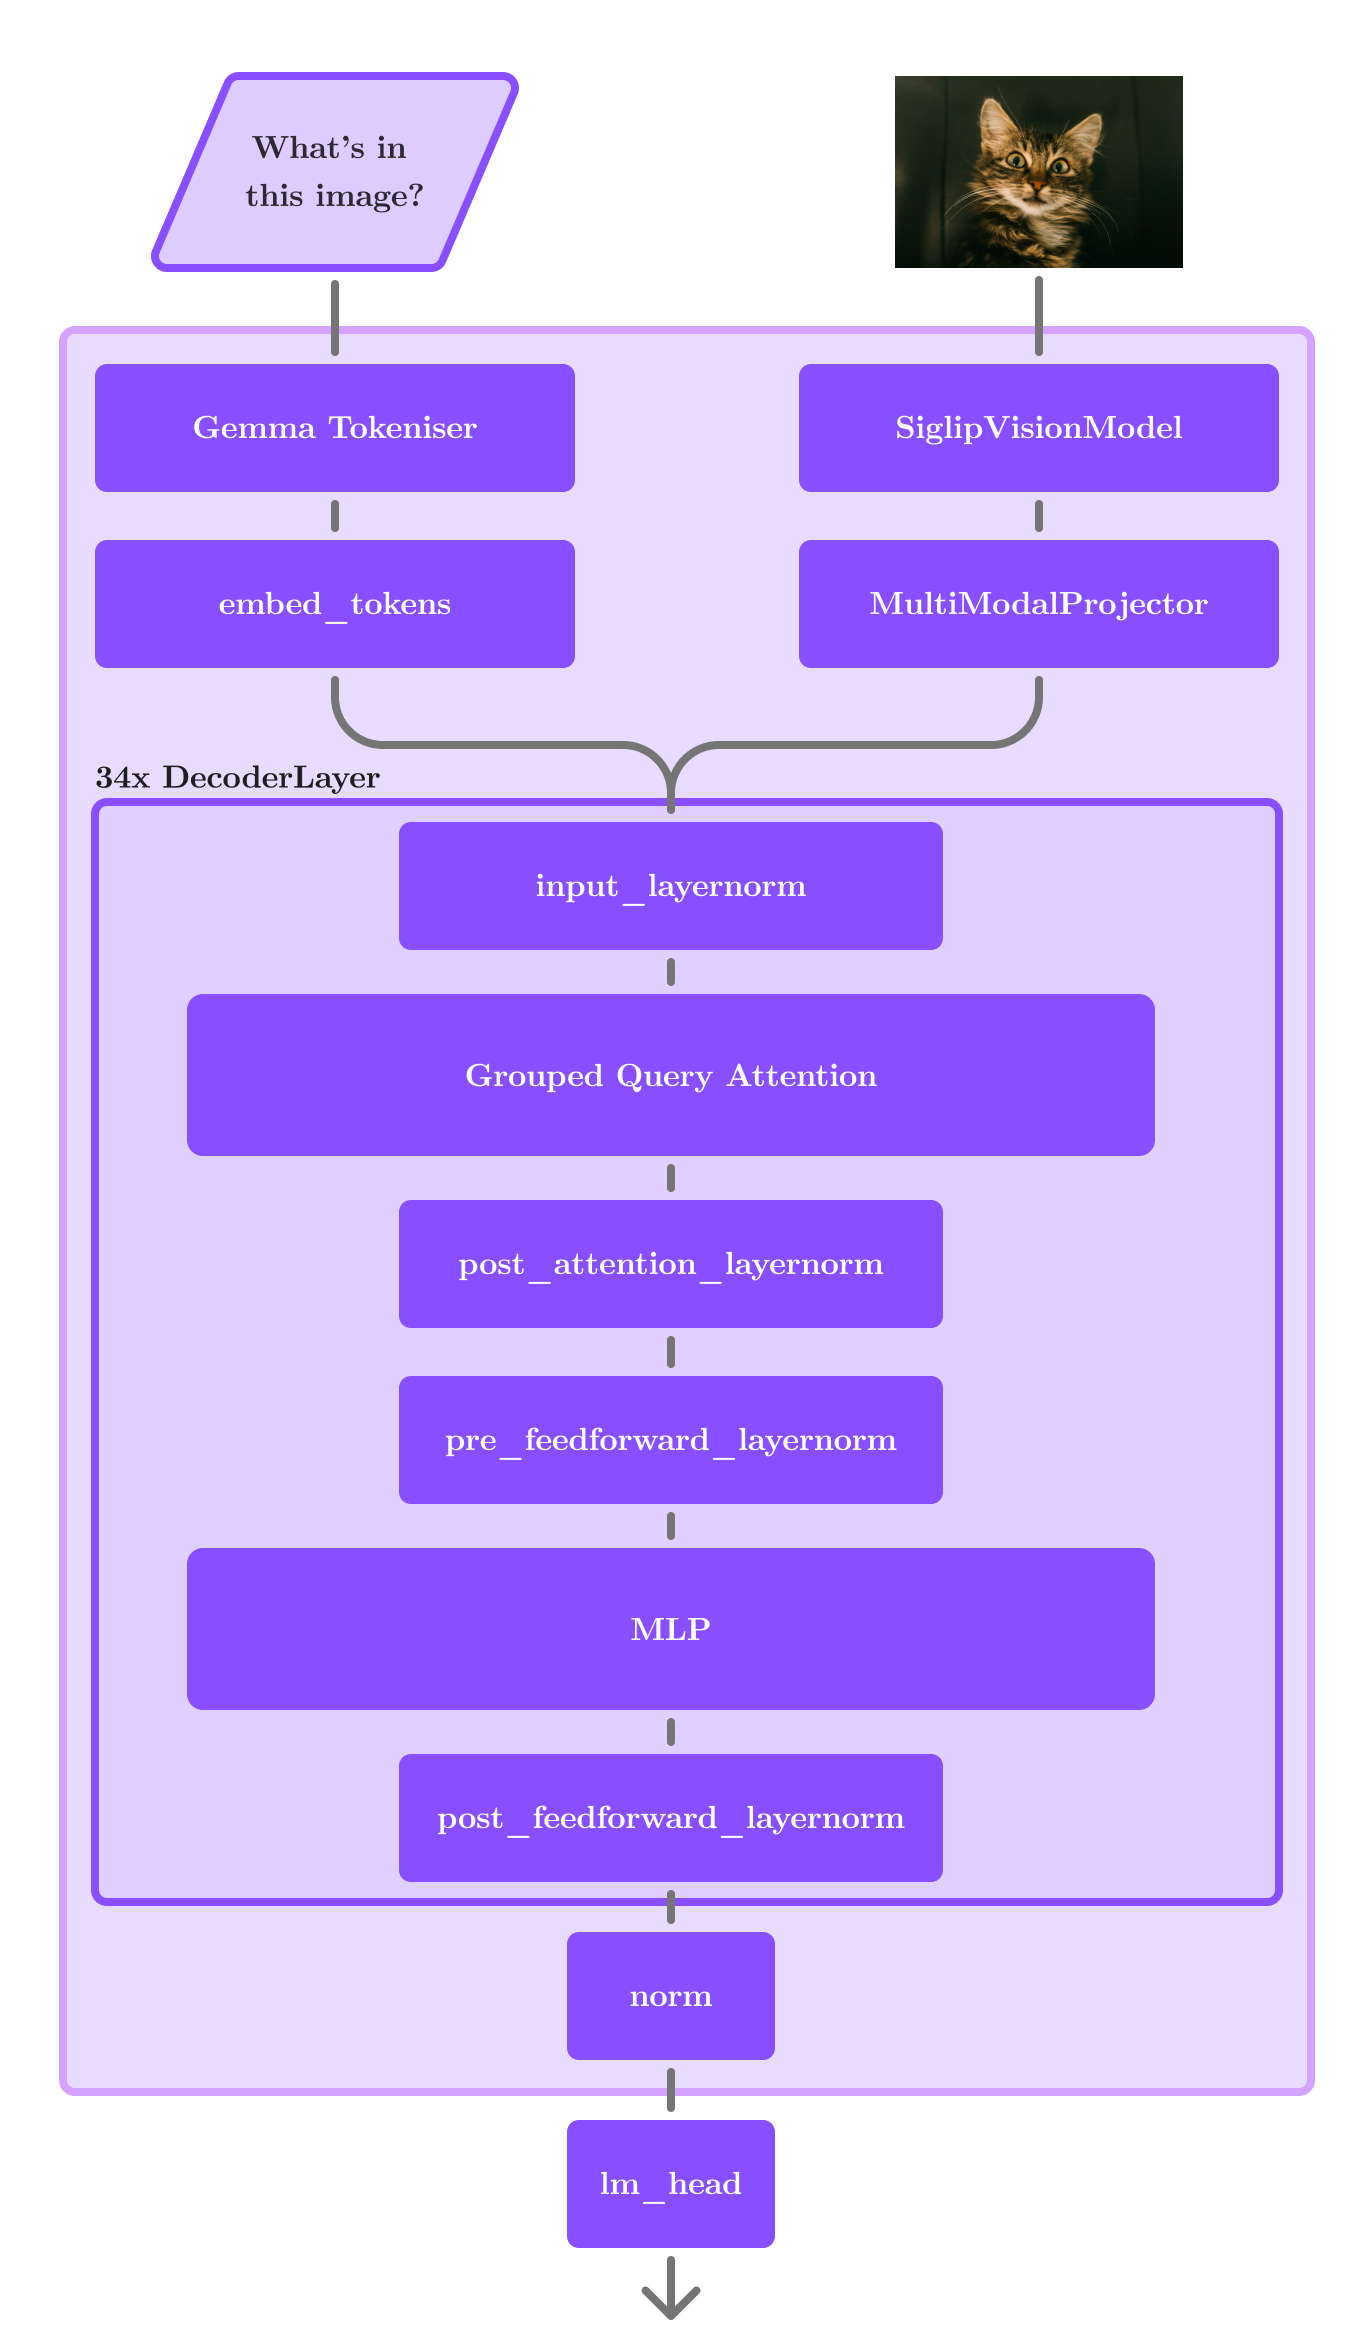
\includegraphics[width=0.75\textwidth]{pages/imgs/vlm/gemma-3-4b-2.png}
	\caption{Architecture diagram of Gemma 3 (4B variant), highlighting the visual encoder, token projector, and decoder with mixed attention.}
	\label{fig:gemma3_arch}
\end{figure}

% \subsubsection{Soft-Target Distillation with Sampled Logits} All Gemma 3 models are trained from scratch using an aggressive knowledge distillation (KD) scheme. Instead of learning only from one-hot ground-truth tokens, the Gemma 3 student models learn from a large teacher model’s full probability distribution at each position. This soft-target distillation approach, pioneered by \citet{hinton2015distilling}, provides a much richer training signal than hard one-hot targets, as it teaches the student not just the correct answer but also the teacher’s confidence in various alternatives. However, directly using the teacher’s complete probability distribution over the vocabulary (of size $|\mathcal{V}|\approx 256$k) at every step would be computationally infeasible. Gemma 3 addresses this by using a sampled soft-target approach. For each training token position, rather than computing the teacher’s full $|\mathcal{V}|$-sized softmax, a subset $U$ of 256 logits is sampled according to the teacher’s output distribution \citep{gemma3}. This subset $U$ includes the few highest-probability tokens (to cover the most likely predictions) and additional tokens sampled in proportion to the teacher’s probability $P_T(v)$, always including the ground-truth token. The teacher’s original probability mass on those 256 tokens is then renormalized to sum to 1, with all other tokens in the vocabulary treated as having zero probability. The student model is trained to predict this teacher-truncated distribution using a cross-entropy loss. Formally, let $P_T(v)$ be the teacher’s probability for token $v$ at a given position, and $P_S(v)$ be the student’s predicted probability. If $U \subset \mathcal{V}$ is the sampled subset of 256 tokens (with the ground-truth included), we define the renormalized teacher distribution on $U$ as $\displaystyle \tilde{P}T(v) = \frac{P_T(v)}{\sum{u \in U} P_T(u)}$. 

% The distillation loss is then defined as:
% \[
% L_{\text{KD}} = - \sum_{v \in U} \tilde{P}_T(v) \log P_S(v)
% \]

% computed only over the tokens in $U$. Here the teacher’s probability for any token not in $U$ is effectively $0$ (since it is “set to zero” and not used), and thus the student is not penalized for those outputs \citep{gemma3}. Over training, different random subsets $U$ are sampled on different occurrences, so the student eventually sees a wide support of the teacher’s distribution.

% This distillation approach significantly boosts the students’ performance: indeed, Gemma 3 models achieve substantially higher performance than Gemma 2 models of equivalent size, thanks to the transferred knowledge from the teacher \citep{gemma3, gemma2}. In other words, using KD allows a smaller Gemma 3 model to approximate the quality of a much larger model, closing the gap in capability that would otherwise exist between model sizes.


\begin{exercise}
As the final exercise, we will implement a function for multimodal tokenization and test multimodal generation with Gemma 3. 
This exercise will guide you through completing the corresponding notebook located at \texttt{lxmls/labs/notebooks/multimodal/vlm\_exercise.ipynb}, focusing on the key steps required to process interleaved image and text data for a VLM.

\begin{enumerate}
    \item \textbf{Setup:}
    Begin by running the first cell in the notebook to import the necessary libraries.

    \item \textbf{Tokenisation without padding using Image Placeholders}\newline
    Your first task is to complete the \texttt{tokenize\_without\_padding} function, which translates a multimodal sequence of text and images into a list of token IDs. Your implementation should:
    \begin{itemize}
        \item Start the token sequence with a single beginning-of-sequence (\texttt{[BOS]}) token.
        \item Iterate through the prompt. If an element is a string, encode it into token IDs. If it is an image, you must insert a specific sequence of special tokens: a newline, a beginning-of-image token, a set of image placeholder tokens, and an end-of-image token. Each of these tokens are accessed as part of the \texttt{Tokenizer} class defined in ``lxmls/multimodal/gemma3/processor.py''.
        \item As hinted in the notebook, the number of placeholder tokens is determined by the architecture of the vision model. It corresponds to the number of feature vectors generated by the SigLIP encoder for each image. Refer to the definition of the SigLIP encoder in ``lxmls/multimodal/gemma3/siglip\_vision/model.py'' and its config in ``lxmls/multimodal/gemma3/siglip\_vision/model.py'' to find this value.
        \item Finally, collect all PIL Images into a separate list to be processed by the vision encoder later.
    \end{itemize}
    \begin{python}
def tokenize_without_padding(
    prompt: Sequence[str | torch.Tensor],
    tokenizer: Tokenizer,
    vis_cfg: SiglipVisionModelConfig,
) -> Tuple[list[int], list[torch.Tensor]]:
    """
    Processes a single preprocessed prompt containing text and image tensors.
    """
    token_ids: List[int] = []
    images: List[torch.Tensor] = []

    # YOUR SOLUTION HERE

    return token_ids, images
    \end{python}

    \item \textbf{Padding the Sequences}\newline
    Most deep learning models process data in batches for efficiency. 
    Since different prompts will have different lengths of text and numbers of images, we must pad them to uniform dimensions.
    \begin{itemize}
        \item Complete the \texttt{pad\_token\_sequences} function to pad each token list to the maximum sequence length in the batch using the tokenizer's \texttt{pad\_id}.
        \item Next, complete the \texttt{pad\_image\_sequences} function. This function should pad the list of images with zero-tensors and create a boolean \texttt{image\_presence\_mask} to differentiate real images from padding.
    \end{itemize}
    \begin{python}
def pad_token_sequences(all_token_ids: List[List[int]], max_seq_len: int, pad_id: int) -> List[List[int]]:
    """
    Pads each token sequence in a batch to a specified maximum length.
    """
    # YOUR SOLUTION HERE
    
    return finalised_token_ids
    
def pad_image_sequences(
    all_images: List[List[torch.Tensor]],
    max_num_images: int,
    vis_cfg: SiglipVisionModelConfig,
    device: Any,
) -> Tuple[List[List[torch.Tensor]], List[List[bool]]]:
    """
    Pads each list of images in a batch to a specified maximum number.
    """
    # YOUR SOLUTION HERE
    
    return image_batch, image_presence_mask
    \end{python}
    
    \item \textbf{Execution and Generation:}
    The notebook provides the main \texttt{tokenize} and \texttt{generate} functions that orchestrate the steps you've implemented.
    \begin{itemize}
        \item Review the logic in these functions to understand how your helper functions are used in the complete pipeline.
        \item Run the final cells to test your implementation. Observe the model's responses to the text-only, single-image, and interleaved prompts. 
        \item How does the model's output for the final prompt demonstrate its ability to ground language in visual context?
    \end{itemize}
    
\end{enumerate}
\end{exercise}